\documentclass[12pt,a4paper,openright,twoside]{report}


\usepackage[british]{babel}
\usepackage[utf8]{inputenc}


\usepackage{fancyhdr}
\usepackage{indentfirst}
\usepackage{graphicx}
\usepackage{newlfont}
\usepackage{xcolor}


\usepackage{amssymb}
\usepackage{amsmath}
\usepackage{latexsym}
\usepackage{amsthm}


\oddsidemargin=30pt 
\evensidemargin=20pt
\hyphenation{sil-la-ba-zio-ne pa-ren-te-si}
\pagestyle{fancy}\addtolength{\headwidth}{20pt}
\renewcommand{\chaptermark}[1]{\markboth{\thechapter.\ #1}{}}
\renewcommand{\sectionmark}[1]{\markright{\thesection \ #1}{}}
\rhead[\fancyplain{}{\bfseries\leftmark}]{\fancyplain{}{\bfseries\thepage}}
\cfoot{}
\linespread{1.3}

% Style theorem boxes

\theoremstyle{plain}
\newtheorem{prop}{Proposition}
\newtheorem{defin}[prop]{Definition}
\newtheorem{intdef}[prop]{(Intuitive) Definition}

\theoremstyle{definition}
\newtheorem{rem}[prop]{Remark}
\newtheorem{ex}[prop]{Example}


%%%%%%%%%%%%%%%%%%%%%%%%% DEDICATION %%%%%%%%%%%%%%%%%%%%%%%%%%%%%%%%%%%%%%%

\begin{document}

\begin{titlepage}
\thispagestyle{empty}                   
\topmargin=6.5cm                        
\raggedleft                             
\large                                  
                                       
\em                                     
To my beloved\\
Benedetta                   
\newpage                                

\clearpage{\pagestyle{empty}\cleardoublepage}
\end{titlepage}
\pagenumbering{roman}


            




%%%%%%%%%%%%%%%%%%%%%%% INTRODUCTION %%%%%%%%%%%%%%%%%%%%%%%%%%%%%%

\chapter*{Introduction}   
\addcontentsline{toc}{chapter}{Introduction}
\rhead[\fancyplain{}{\bfseries Introduction}]{\fancyplain{}{\bfseries\thepage}}\lhead[\fancyplain{}{\bfseries\thepage}]{\fancyplain{}{\bfseries Introduction}}




  \textcolor{blue}{Machine learning literature is exploding in size and complexity, but most solutions found are ad hoc, there is little communication between different subfields, and there is a large research debt. Category theory can solve these problems.  \cite{shieblerCategoryTheoryMachine2021}.}

  \textcolor{blue}{Talk about the origins of category theory and its "rise to power" as a common language that aims to unite different fields of knowledge.}
    
  \textcolor{blue}{Discuss the purpose of this work: a beginner-friendly survey of categorical approaches to neural networks, causal models, and interpretability.}





%%%%%%%%%%%%%%%%%%%%%%% ITALIAN TRANSLATION OF THE INTRODUCTION %%%%%%%%%%%%%%%%%%%%%%%%%%%%%%


\chapter*{Introduzione}
\addcontentsline{toc}{chapter}{Introduzione}
\rhead[\fancyplain{}{\bfseries Introduzione}]{\fancyplain{}{\bfseries\thepage}}\lhead[\fancyplain{}{\bfseries\thepage}]{\fancyplain{}{\bfseries Introduzione}}





  \textcolor{blue}{Traduzione italiana dell'introduzione.}







%\clearpage{\pagestyle{empty}\cleardoublepage}


%%%%%%%%%%%%%%%%%%%%%%%%%%%%% TABLE OF CONTENTS %%%%%%%%%%%%%%%%%%%%%%%%%%%%%%

\tableofcontents
\rhead[\fancyplain{}{\bfseries\leftmark}]{\fancyplain{}{\bfseries\thepage}} \lhead[\fancyplain{}{\bfseries\thepage}]{\fancyplain{}{\bfseries Table of Contents}}
%\clearpage{\pagestyle{empty}\cleardoublepage}

\listoffigures                         
%\clearpage{\pagestyle{empty}\cleardoublepage}


\listoftables                           
%\clearpage{\pagestyle{empty}\cleardoublepage}





%%%%%%%%%%%%%%%%%%%%%%%%% CATEGORICAL TOOLKIT %%%%%%%%%%%%%%%%%%%%%%%%%%%%%


\chapter{Categorical Toolkit}
\lhead[\fancyplain{}{\bfseries\thepage}]{\fancyplain{}{\bfseries\rightmark}}
\pagenumbering{arabic}



\textcolor{blue}{Brief introduction to category theory and the categorical toolkit used in the following sections. As each kind of category is introduced we shall also introduce appropriate string diagrams.}



  \section{Basics of Category Theory}


  \textcolor{blue}{Definition of category.}
  \textcolor{blue}{Definition of functor.}
  \textcolor{blue}{Definition of natural transformation.}
  \textcolor{blue}{Definition of 2-category.}


  \section{Various Families of Categories}

  \subsection{Monoidal Categories}

  \textcolor{blue}{Definition of monoidal category.}
  \textcolor{blue}{Definition of Cartesian category.}
  \textcolor{blue}{Expand on the properties of Cartesian categories. In particular, expand on the existence of copy maps.}
  \textcolor{blue}{Definition of left-additive category.}
  \textcolor{blue}{Definition of Cartesian left-additive category.}




  \subsection{Differential Categories}

  The recent rise in AI techniques was only possible because of advancements in automatic differentiation (AD) techniques. Differentiation in machine learning is usually carried out in Euclidean spaces $\mathbb{R}^n$, but is worth considering more abstract settings because the techniques used in gradient-based learning can be greatly generalized. For instance, \cite{wilsonReverseDerivativeAscent2021a} demonstrated that gradient-based learning can take place in the context of Boolean circuits.


  We consider two abstract settings for differentiation: Cartesian differential categories (first introduced in \cite{bluteDifferentialCategories2006}) and Cartesian reverse differential categories (first introduced by \cite{cockettReverseDerivativeCategories2019}). The former is a setting where forward derivatives of morphisms can be taken, while the latter is a setting where reverse derivatives can be taken. We shall only give intuitive definitions for the sake of brevity; rigorous definition which account of all the necessary axioms can be found in \cite{cockettReverseDerivativeCategories2019}.

  \begin{intdef}[Cartesian differential category]
    A Cartesian differential category (CDR) $\mathcal{C}$ is a Cartesian left-additive category where a differential combinator $\mathrm{D}$ is defined. Such differential combinator must take a morphism $f: A \to B$ and return a morphism $\mathrm{D}[f]: A \times A \to B$, which is known as the derivative of $f$. The combinator $\mathrm{D}$ must satisfy a number of axioms. 
  \end{intdef}

  \begin{intdef}[Cartesian reverse differential category]
    A Cartesian reverse differential category (CRDC) $\mathcal{C}$ is a Cartesian left-additive category where a reverse differential combinator $\mathrm{R}$ is defined. Such reverse differential combinator must take a morphism $f: A \to B$ and return a morphism $\mathrm{R}[f]: A \times B \to A$, which is known as the reverse derivative of $f$. The combinator $\mathrm{R}$ must satisfy a number of axioms. 
  \end{intdef}

  
  The aforementioned axioms make sure that $\mathrm{R}$ and $\mathrm{D}$ satisfy the properties expected from derivative and reverse derivative. In particular, a differential combinator satisfies a chain rule (see figure ADDIM), whereas a reverse differential combinator satisfies a reverse chain rule (see figure ADDIM).

  
  \begin{ex}
    $\mathbf{Smooth}$ is a both a CDC and a CRDC. In fact, if $\mathcal{J}_f$ is the Jacobian matrix of a smooth morphism $f$,
    \[\mathrm{D}[f]: (x,v) \mapsto \mathcal{J}_f(x)v\]
    and
    \[\mathrm{R}[f]: (x,y) \mapsto \mathcal{J}_f(x)^Ty\]
    induce well-defined combinators $\mathrm{D}$ and $\mathrm{R}$. This is only a partial coincidence, as it is shown in \cite{cockettReverseDerivativeCategories2019} that CRDCs are always CDCs under a canonical choice of differential combinator. The converse, however, is generally false.
  \end{ex}



  \subsection{Lenses}\label{subsec: lenses}

  Lenses are a mathematical construct used to model bidirectional flows of information\footnote{The theory of optics generalizes lenses to a much wider family of constructs that model these same bidirectional flows. See \cite{rileyCategoriesOptics2018}.}. Such flows are extremely important in machine learning as a machine learning model needs both to carry out a computation and to update its parameters based on the training data.

  \begin{defin}[Lenses]
    Let $\mathcal{C}$ be a Cartesian category. We define $\mathbf{Lens}(\mathcal{C})$ as the category constituted by the following objects and morphisms.
    An object of $\mathbf{Lens}(\mathcal{C})$ is a pair $\left(\begin{smallmatrix} A \\ A' \end{smallmatrix}\right)$ of objects in $\mathcal{C}$; 
    A $\left(\begin{smallmatrix} A \\ A' \end{smallmatrix}\right) \to \left(\begin{smallmatrix} B \\ B' \end{smallmatrix}\right)$ morphism (or lens) is a pair $\left(\begin{smallmatrix} f \\ f^* \end{smallmatrix}\right)$ of morphisms of $\mathcal{C}$ such that $f: A \to B$ and $f^*: A \times A'$. $f$ is known as get part of the lens $\left(\begin{smallmatrix} f \\ f^* \end{smallmatrix}\right)$, whereas $f^*$ is known as get part. Given a pair $\left(\begin{smallmatrix} A \\ A' \end{smallmatrix}\right)$, the associated identical lens is $\left(\begin{smallmatrix} 1_A \\ \pi_1 \end{smallmatrix}\right)$. Lens composition is illustrated by ADDIM.
  \end{defin}

  Lenses can be represented using the language string diagrams (see \cite{cruttwellDeepLearningParametric}), both in compact form and in expanded form.


  It is important to note the following (see \cite{cruttwellDeepLearningParametric}):
  
  \begin{prop}
    If $\mathcal{C}$ is a Cartesian category, $\mathbf{Lens}(\mathcal{C})$ is a monoidal category under the monoidal product $\left(\begin{smallmatrix} A \\ A' \end{smallmatrix}\right) \otimes \left(\begin{smallmatrix} B \\ B' \end{smallmatrix}\right) = \left(\begin{smallmatrix} A \times B \\ A' \times B' \end{smallmatrix}\right)$.
  \end{prop}

  Another important result from \cite{cruttwellDeepLearningParametric} is (according the formulation found in \cite{shieblerCategoryTheoryMachine2021}):

  \begin{prop}\label{prop: canembedding1}
    If $\mathcal{C}$ is a CRDC, there exists a canonical Cartesian left-additive functor $R_\mathcal{C}$ which embeds $\mathcal{C} \to \mathbf{Lens}(\mathcal{C})$. Such functor maps objects as $A \mapsto \left(\begin{smallmatrix}A \\ A\end{smallmatrix}\right)$ and maps morphisms as $f \mapsto \left(\begin{smallmatrix}f \\ \mathrm{R}[f]\end{smallmatrix}\right)$.
  \end{prop}

  \begin{rem}
    Consider the put map of the composition of two lenses, as in figure ADDIM. As \cite{shieblerCategoryTheoryMachine2021} notes, there is a striking resemblance between the form that such put map takes and the reverse chain rule that holds in a CRDC. This similarity will be important for modelling neural networks as lenses. 
  \end{rem}




  \subsection{The $\mathbf{Para}$ Construction}\label{subsec: para}


  In machine learning, it is often necessary to work with parameters. Although lenses can model bidirectional flow, they don't afford us the machinery needed to work with such parameters. The $\mathbf{Para}$ construction allows us to overcome such limit. For the sake of simplicity, we shall only examine the case where parameters and values are taken from the same category $\mathcal{C}$ (as in \cite{cruttwellDeepLearningParametric}). A more general $\mathbf{Para}$ construction is described in \cite{shieblerCategoryTheoryMachine2021}, where actegories are used to handle a much wider choice of possible parameters.

  \begin{intdef}[$\mathbf{Para}(\mathcal{C})$]
    Let $(\mathcal{C},I,\otimes)$ be a symmetric monoidal category. Then, we define $\mathbf{Para}(\mathcal{C})$ as the $2$-category whose components are as follows.
    \begin{itemize}
      \item The $0$-cells are the objects of $\mathcal{C}$.
      \item The $1$-cells are pairs $(P,f): A \to B$, where $P \in \mathcal{C}$ and $f: P \otimes A \to B$.
      \item The $2$-cells come in the form $r: (P,f) \to (Q,g)$, where $r: P \to Q$ is a morphism in $\mathcal{C}$. $r$ must also satisfy a naturality condition.
      \item The $1$-cell identity on $A$ in $\mathbf{Para}(\mathcal{C})$ is $(I,1_A)$.
      \item The $2$-cell identity on $(P,f)$ in $\mathbf{Para}(\mathcal{C})$ is $1_P$.
      \item The $1$-cell composition law is
        \[(P,f) ; (Q,g) = (Q \otimes P, Q \otimes f ; g.\]
      \item The $2$-cell composition law is the same as the $\mathcal{C}$ composition law.
    \end{itemize}
     
  \end{intdef}

  The intuition behind the definition above is the following: the $1$ cells are parametric maps, whereas the $2$ cells are reparametrisations.
  It is quite handy to represent such cells using the string diagram notation illustrated in figure ADDIM.
  
  
  The category of parametric lenses associated with a given Cartesian left-additive category $\mathcal{C}$, i.e. $\mathbf{Para}(\mathbf{Lens}(\mathcal{C}))$ is particularly significant. It is shown in \cite{cruttwellDeepLearningParametric} that $\mathbf{Para}(\mathcal{C})$ is natural with respect to $\mathcal{C}$. In other words, as emphasized in \cite{shieblerCategoryTheoryMachine2021},
  
  \begin{prop}\label{prop: canembedding2}
    If $\mathcal{C}$ and $\mathcal{D}$ are symmetric monoidal categories and $F: \mathcal{C} \to \mathcal{D}$ is a symmetric monoidal functor, then  there is a canonical $2$-functor 
    \[\mathbf{Para}(F): \mathbf{Para}(\mathcal{C}) \to \mathbf{Para}(\mathcal{D}).\]
  \end{prop}

  Refer to \textit{Fig. ADDIM} to see a string diagram that shows the inner workings of a parametric lens.






  %\begin{figure}[h]
  %  \begin{center}                         
  %    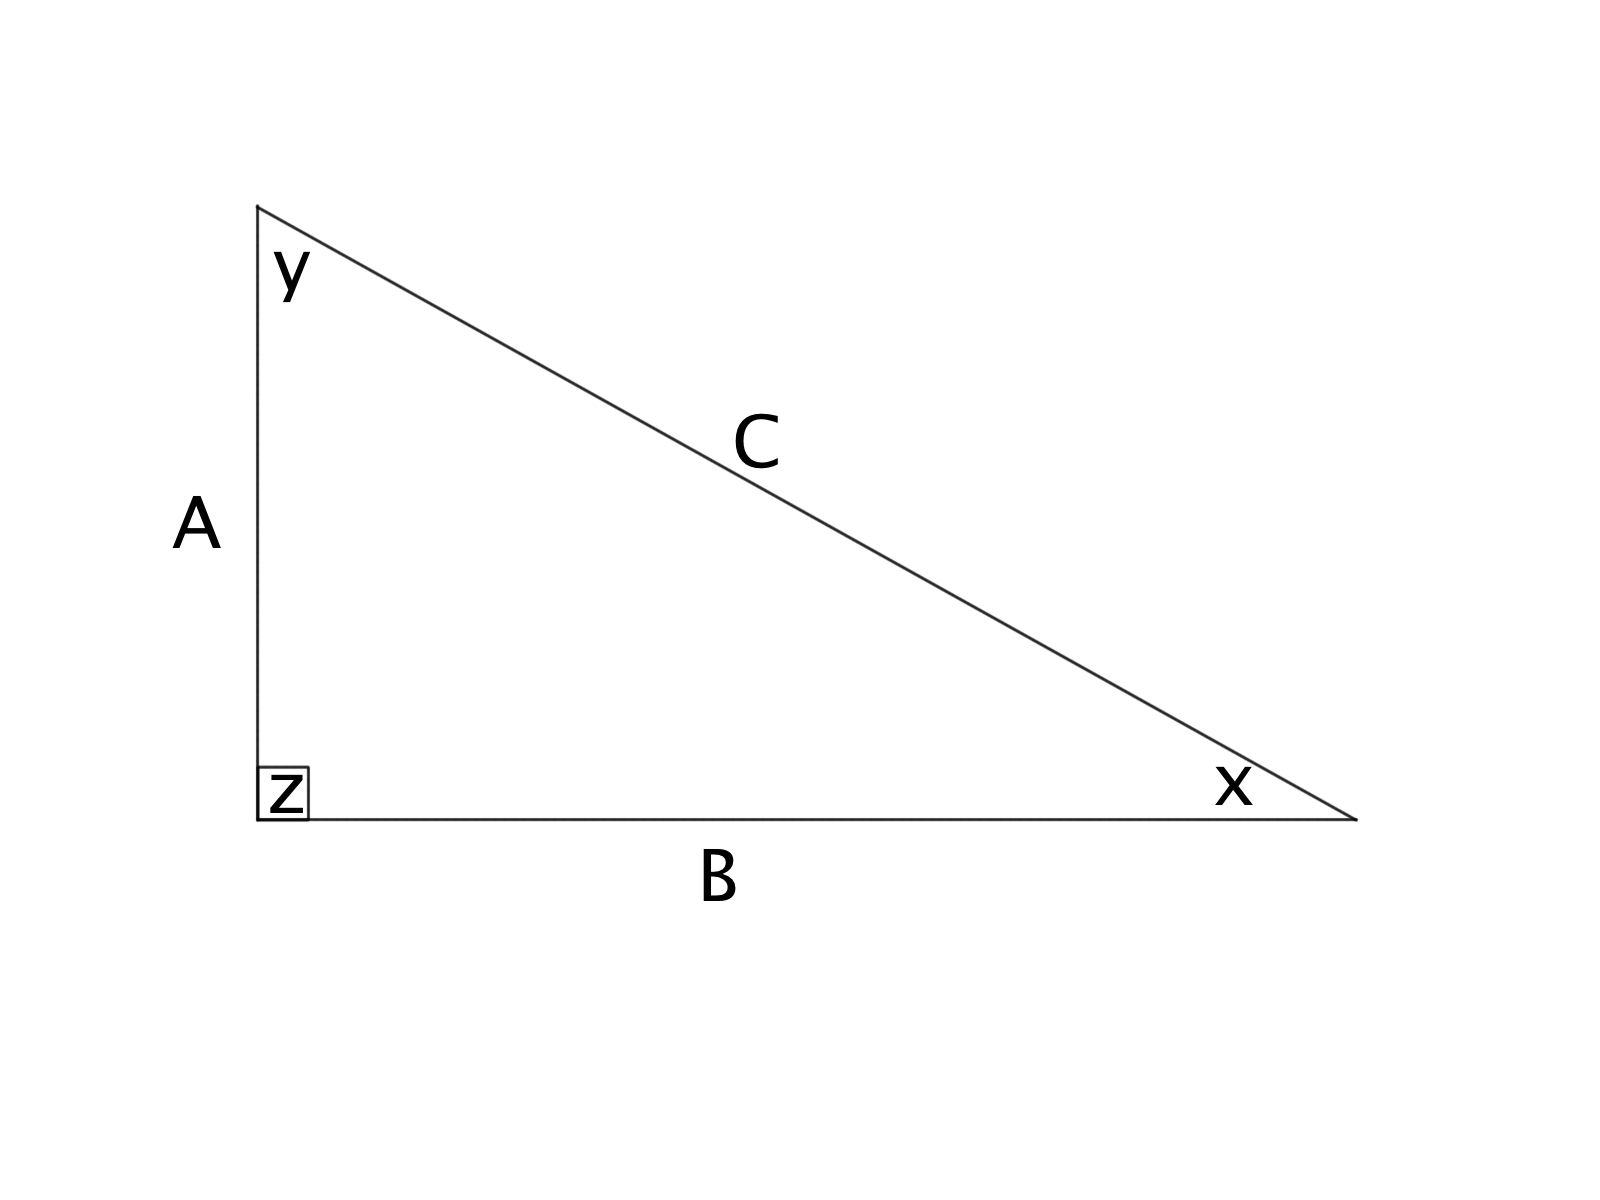
\includegraphics[width=5cm]{figures/triangle.jpg}
  %    \caption[Placeholder]{Placeholder figure.}\label{fig:first}
  %  \end{center}
  %\end{figure}

  %\begin{table}[h]                        
  %  \begin{center}                          
  %    \begin{tabular}{r|c|c}                  
  %      \hline \hline                           
  %      $(1,1)$ & $(1,2)$ & $(1,3)$\\           
  %      \hline                                  
  %      $(2,1)$ & $(2,2)$ & $(2,3)$\\           
  %      \hline                                  
  %      $(3,1)$ & $(3,2)$ & $(3,3)$\\
  %      \hline \hline                           
  %    \end{tabular}
  %    \caption[Placeholder Table]{Placeholder table.}\label{tab:uno}
  %  \end{center}
  %\end{table}



%%%%%%%%%%%%%%%%%%%%%%% CATEGORICAL APPROACHES TO NNS %%%%%%%%%%%%%%%%%%%%%%%%%%%


\chapter{Categorical Approaches to Neural Networks}
\lhead[\fancyplain{}{\bfseries\thepage}]{\fancyplain{}{\bfseries\rightmark}}




\textcolor{blue}{Brief summary of the chapter.}





\section{Learning with Parametric Lenses}


Pretrained neural networks can be though of as differentiable functions between Euclidean spaces, but a more sophisticated model is needed if we want to study the training process in its entirety. A neural network that needs to be trained is best thought of as a parametric map: training means finding the best parameters for the task at hand. Thus, it makes sense to represent layers of a neural network as parametric maps in $(P,f) \in \mathbf{Para}(\mathcal{C})(A,B)$, for some symmetric monoidal category $\mathcal{C}$.


The process of training, however, requires a bidirectional flow of information: we have to test the current parameters and apply some criterion to find new parameters that (hopefully) satisfy the requirements better. In gradient based learning, the aforementioned criterion requires computing the gradient of the loss function using specialized algorithms such as backpropagation. It has been shown numerous time (see e.g. ADDREF) that taking the reverse derivative instead of the forward derivative is more efficient for functions with lower dimensionality in the codomain, which is commonplace in real word neural networks. Hence, it makes sense to require $\mathcal{C}$ to be CRDC. 

The position held by \cite{cruttwellDeepLearningParametric} is that the most natural way to relate forward and backward propagation of information in neural network is to represent the components of the network as parametric lenses where the get map handles forward propragation while the put map handles backward propagation. For instance,  in place of $(P,f)$, we would consider
\begin{equation}
  \label{eq: exparametriclens}
  \left(\begin{pmatrix} P \\ P \end{pmatrix},\begin{pmatrix} f \\ \mathrm{R}[f] \end{pmatrix}\right) 
  \in \mathbf{Para}(\mathbf{Lens}(\mathcal{C}))
  \left(\begin{pmatrix} A \\ A \end{pmatrix},\begin{pmatrix} B \\ B \end{pmatrix}\right).
\end{equation}
The authors of \cite{cruttwellDeepLearningParametric} take this line of reasoning a step further and show that it is also meaningful to represent other components of learning - such as optimizers, loss functions, and learning rates - within the framework of parametric lenses. 

The main insight that makes parametric lenses as the one above useful is contained in \textit{Prop. \ref{prop: canembedding1}} and \textit{Prop. \ref{prop: canembedding2}}. If $\mathcal{C}$ is CRDC, we can functorially embed $\mathcal{C}$ into $\mathbf{Lens}(\mathcal{C})$ by considering lenses whose put map is the reverse derivative of the get map. Moreover, we can functorially embed $\mathbf{Para}(\mathcal{C})$ into $\mathbf{Para}(\mathbf{Lens}(\mathcal{C}))$ with the same exact "trick". Hence, lenses as the one in \textit{Eq. \ref{eq: exparametriclens}} are compositional. In addition, (i) the get map of the composition of two lenses is the composition of the get maps, (ii) the put map of the composite lens is the reverse derivative of the composition of the put maps. Hence, if $\left(\left(\begin{smallmatrix} P \\ P \end{smallmatrix}\right),\left(\begin{smallmatrix} f \\ \mathrm{R}[f] \end{smallmatrix}\right)\right)$ represents a linear layer and $\left(\left(\begin{smallmatrix} Q \\ Q \end{smallmatrix}\right),\left(\begin{smallmatrix} g \\ \mathrm{R}[g] \end{smallmatrix}\right)\right)$ represents an activation layer, their composition represents a fully connected layer according to the same convention.



Surprisingly, even loss maps can be represented as parametric maps and thus as parametric lenses.
For instance, we may represent a loss maps as $(P,\mathrm{loss}) \in \mathbf{Para}(\mathcal{C})(B,L)$ for some object $L$. The intuitive meaning of this representation is the following: $\mathrm{loss}$ takes the output of the network of type $B$, compares it with the labels of type $P$ ($P$ and $B$ will often coincide in practical examples), and then returns a loss of type $L$. The parametric lens associated with $\mathrm{loss}$ can thus be post-composed after the parametric lens associated with a neural network to compute the loss generated by such network given some input and the associated labels. This process is illustrated in Fig. ADDIM.


This leaves two dangling wires of type $L$. We can use a learning rate lens $\alpha$ to link the wires and allow forward-propagating information to "change direction" and go backwards. $\alpha$ must have domain equal to $\left( \begin{smallmatrix} L \\ L \end{smallmatrix} \right)$ and codomain equal to $\left(\begin{smallmatrix} 1 \\ 1 \end{smallmatrix}\right)$, where $1$ is the terminal object of $\mathcal{C}$. For instance, if $\mathcal{C} = \mathbf{Smooth}$, $\alpha$ might just multiply the loss by some $\epsilon$, which is what machine learning practitioners would ordinarily call learning rate. Fig. ADDIM shows how a learning rate can be linked to the loss function and the model using post-composition.


The final element needed for the model $f$ in Fig. ADDIM to learn is an optimizer. It is shown in \cite{cruttwellDeepLearningParametric} that optimizers can be represented as reparametrisations in $\mathbf{Para}(\mathbf{Lens}(\mathcal{C}))$. More specifically, we might see an optimizer as a lens $\left( \begin{smallmatrix} P \\ P \end{smallmatrix} \right) \to \left( \begin{smallmatrix} Q \\ Q \end{smallmatrix} \right)$. In gradient descent, for example, $P = Q$ and the aforementioned lens is $\left( \begin{smallmatrix} 1_P \\ +_P \end{smallmatrix} \right)$. We can plug such reparametrisation on top of the model to obtain the string diagram in Fig. ADDIM. The diagram shows how the machinery hidden by the $\mathbf{Para}(\mathbf{Lens}(\mathcal{C}))$ can take care of forward propagation, loss computation, backpropagation and parameter updating in a seamless fashion. This is the true power of the compositional mindset: abstraction hides away unwanted detail so that one can focus on high-level features of the model without worrying about side-effects.


The authors of \cite{cruttwellDeepLearningParametric} go on to show that their compositional framework can handle a number of non-trivial deep learning architectures such as CNNs, GANs, and deep dreaming. For instance, the copy maps of CRDCs can model weight sharing and batching, and even a whole learning iteration can be represented as a large string diagram. Finally, the authors prove that the compositional point of view afforded by parametric lenses is of practical significance by implementing a proof-of-concept Python library. The library is then used to build a model able to classfy MNIST. In their words, \lq[the] proposed algebraic structures naturally guide programming practice\rq.


\begin{rem}
  We have presented the perspective of \cite{cruttwellDeepLearningParametric} within the context of neural networks for the sake of simplicity, but the tools introduced in the paper apply to a much wider context. For instance, it is show in \cite{wilsonCategoriesDifferentiablePolynomial2022} that polynomial circuits form a CRDC, and it is shown in \cite{wilsonReverseDerivativeAscent2021a} that meaningful learning can be carried out in the context of Boolean circuits, as long as a suitable optimizer is chosen. Since the notions is \cite{cruttwellDeepLearningParametric} are developed from the point of view of a generic CRDC - of which $\mathbf{Smooth}$ is just one example - all the above applies to training such networks. This is the advantage of working in an abstract categorical setting. 
\end{rem}


\begin{rem}[Learners]
  One of the first compositional approaches to training neural networks in the literature can be found in the seminal paper ADDREF. The authors introduce a category of learners, objects which are meant to represent components of a neural network and behave similarly as parametric lenses do. The main difference is that each learner is endowed with its own loss map and optimizer. It is argued in \cite{cruttwellDeepLearningParametric} and ADDREF that the perspective \cite{cruttwellDeepLearningParametric} is more flexible than and largely subsumes the learner approach. 
\end{rem}








%\clearpage{\pagestyle{empty}\cleardoublepage}

%%%%%%%%%%%%%%%%%%%%%%%%%%%%%% CONCLUSIONS %%%%%%%%%%%%%%%%%%%%%%%%%%%%%%%%%%%

\chapter*{Conclusions}
\rhead[\fancyplain{}{\bfseries
Conclusions}]{\fancyplain{}{\bfseries\thepage}}
\lhead[\fancyplain{}{\bfseries\thepage}]{\fancyplain{}{\bfseries Conclusions}}
\addcontentsline{toc}{chapter}{Conclusions} 










%%%%%%%%%%%%%%%%%%%%%%%%%%%%%%%%%%%%% BIBLIOGRAPHY %%%%%%%%%%%%%%%%%%%%%%%%%%%%%%

\bibliographystyle{alpha}
\bibliography{references}
\rhead[\fancyplain{}{\bfseries \:Bibliography}]{\fancyplain{}{\bfseries\thepage}} 
\addcontentsline{toc}{chapter}{Bibliography}



% \clearpage{\pagestyle{empty}\cleardoublepage}



%%%%%%%%%%%%%%%%%%%%%%%%%%%%%%%%%%%%%%% ACKNOWLEDGEMENTS %%%%%%%%%%%%%%%%%%%%%%%%%%%

\chapter*{Acknowledgements}

\thispagestyle{empty}

  Placeholder 



\end{document}
